\section{Intelligence Artificielle}

\subsection{CNN}

 Nous avons décidé d'implémenter en premier lieu un modèle CNN (Convolutional Neural Network). Ce type de modèle est adapté aux données séquentilles comme celles que nous possedons. Les CNN peuvent apprendre automatiquement des caractéristiques intéressante pour classifier les données. Ici ils peuvent identifier des motifs spatiaux et temporels. Pour nous aider à implémenter ce modèle, nous nous sommes aidé de keras et en particulier d'un article sur la documentation "Timeseries classification from scratch" \cite{keras} (expliquer ce qu'est keras) Grâce à cet exemple de code nous avons pu élaborer un programme qui entraine un modèle cnn. Tout d'abord il charge les données et les labels a utiliser. Ici nous avons 1312 fichiers à utiliser qui représentent 7 classes (speed\_bump,crack,hole,tree\_bumps,bumpy\_tiles,hole+crack+bumps,speed\_bump+hole). Il sépare les données en entrainement et test avec un pourcentage de 70\% pour l'entrainement et 30\% pour les test. Ici 918 fichiers seront utilisés pour l'entrainement. Enfin le modele cnn a comme architecture l'architecture suivante:
 \begin{figure}[H]
     \centering
     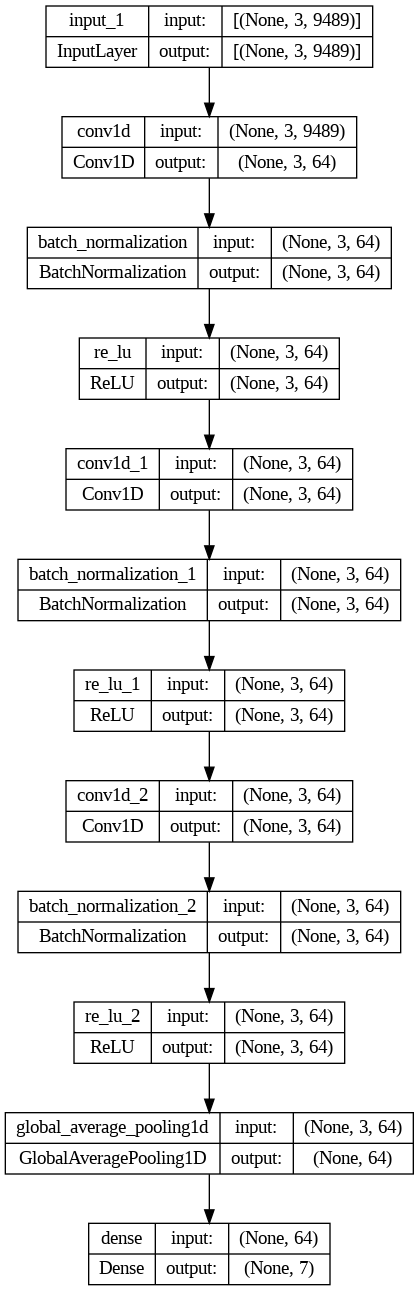
\includegraphics[width=0.4\linewidth]{cnn_pi.png}
     \caption{Architecture du modèle CNN}
     \label{cnn}
 \end{figure}
\newpage
 En utilisant trois couches de convolution avec des noyaux de taille 3 et des filtres de 64, nous pouvons capturer des motifs locaux significatifs dans les données. La normalisation par lots et la fonction d'activation ReLU sont appliquées après chaque couche de convolution pour stabiliser l'entraînement et introduire de la non-linéarité. Le Global Average Pooling est utilisé pour réduire la dimensionnalité des caractéristiques extraites tout en préservant leur pertinence. Enfin, la couche de sortie avec une activation softmax nous permet de classifier les dégradations en différentes catégories. 

Pour l'entraînement de notre modèle, nous avons configuré plusieurs paramètres. Nous avons décidé d'effectuer 500 époques d'entraînement, chacune avec un lot de 32 échantillons. Pour garantir un bon apprentissage, nous avons utilisé trois callbacks. Le premier, "ModelCheckpoint," sauvegarde le modèle qui obtient la meilleure performance sur la perte de validation. Le deuxième, "ReduceLROnPlateau," ajuste automatiquement le taux d'apprentissage si la perte de validation ne s'améliore pas depuis 20 époques. Enfin, le troisième, "EarlyStopping," arrête l'entraînement si la perte de validation ne s'améliore pas pendant 50 époques consécutives. Notre modèle a été compilé avec l'optimiseur "adam" et la perte "sparse\_categorical\_crossentropy" pour la classification, avec une métrique de suivi de la précision "sparse\_categorical\_accuracy". L'entraînement a été effectué sur les données d'entraînement, en utilisant le batch size spécifié, avec 20\% des données réservées à la validation. L'historique de l'entraînement est stocké dans la variable "history" pour une analyse ultérieure. Ces paramètres et callbacks contribuent à un entraînement efficace tout en évitant le surapprentissage grâce à une régularisation adaptée.

Grâce à cet entrainement, nous obtenons un modèle enregistré dans "best\_model.h5" qui atteint une accuracy de 93\% et une loss de 17\% ce qui est très encourageant pour la suite.
\begin{figure}[H]
    \centering
    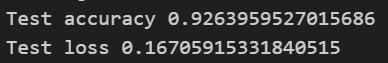
\includegraphics[width=0.5\linewidth]{test.png}
    \caption{Résultats de l'évaluation du modèle CNN}
    \label{resultat_cnn}
\end{figure}

\begin{figure}[H]
    \centering
    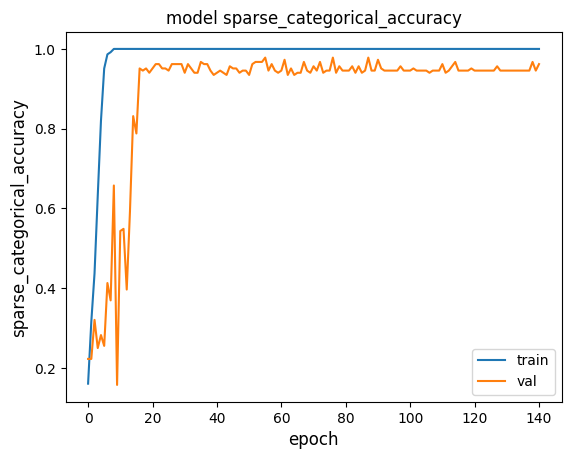
\includegraphics[width=0.5\linewidth]{output.png}
    \caption{Evolution de l'accuracy en fonction des epochs}
    \label{plot_accuracy}
\end{figure}

Voici un exemple d'un résultat donné par le modèle à partir d'une entrée donnée aléatoirement: 
\begin{figure}[H]
    \centering
    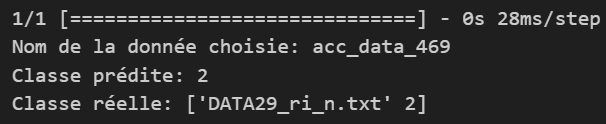
\includegraphics[width=0.5\linewidth]{rescnn.png}
    \caption{Résultat d'une classification du modèle CNN}
    \label{rescnn}
\end{figure}
Ici la donnée en entrée est un fichier contenant les données accélérométriques correspondant à un trou (classe 2), qui a été renversé dans le temps et dans l'espace (ri) et auquel on a rajouté du bruit (n). Le modèle classifie bien cette entrée comme un trou (classe prédite 2).

\subsection{Utilisation du modèle}


\subsection{Implémentation du Modèle LSTM}
Après avoir exploré l'architecture du modèle Convolutional Neural Network (CNN) pour la classification des obstacles, nous avons également développé un modèle basé sur Long Short-Term Memory (LSTM) pour cette tâche. Les réseaux LSTM sont particulièrement adaptés à la modélisation de séquences, ce qui les rend appropriés pour notre problème de classification basée sur des données séquentielles provenant de capteurs embarqués.

\subsubsection{Prétraitement des Données}
Avant de plonger dans les détails du modèle LSTM, nous avons commencé par prétraiter les données d'entrée et de sortie. Les données brutes se composent de séquences de mesures provenant de capteurs inertiels, accompagnées d'étiquettes de classe correspondantes. Les étapes de prétraitement comprenaient :
\begin{itemize}
  \item Conversion des noms de fichiers en valeurs numériques pour un traitement plus facile.
  \item Encodage des étiquettes de classe en utilisant LabelEncoder pour les convertir en valeurs numériques.
  \item Création de séquences de données de longueur uniforme en ajoutant un rembourrage (padding) aux séquences plus courtes.
\end{itemize}

\subsubsection{Création du Jeu de Données}
Nous avons divisé nos données en ensembles d'entraînement et de test en utilisant la fonction \texttt{train\_test\_split} de scikit-learn. Cela nous a permis de disposer d'un ensemble d'entraînement pour former notre modèle LSTM et d'un ensemble de test pour évaluer ses performances.

\subsubsection{Architecture du Modèle LSTM}
Le modèle LSTM est construit en utilisant PyTorch. Il comporte plusieurs couches, notamment une couche LSTM avec des paramètres tels que le nombre de fonctionnalités en entrée, le nombre de couches cachées, et un taux de dropout pour régulariser le modèle. La sortie de la couche LSTM est ensuite envoyée à une couche entièrement connectée (Linear) pour la classification finale.

Le modèle est défini dans la classe \texttt{SequenceModel}, qui est encapsulée dans la classe \texttt{ObstaclePredictor}. Cette dernière est responsable de la formation, de la validation et des prédictions du modèle LSTM.

\subsubsection{Fonction de Perte et Métriques d'Évaluation}
La fonction de perte utilisée pour l'apprentissage est la CrossEntropyLoss, qui est adaptée à la classification multiclasse. Pour évaluer les performances du modèle, nous avons utilisé la métrique de précision pondérée, calculée à l'aide de la bibliothèque TorchMetrics.

\subsubsection{Entraînement et Évaluation du Modèle}
Nous avons essayé de lancer l'entraînement du modèle LSTM sur plusieurs époques à l'aide du module PyTorch Lightning. Cependant une erreur technique nous a empêcher d'évaluer les performances du modèle.\\

L'implémentation du modèle LSTM pour la classification des obstacles basée sur des données séquentielles s'est avérée être un défi complexe et a rencontré des difficultés lors de l'exécution. Malheureusement, le modèle n'a pas pu être correctement formé en raison de certaines erreurs techniques.\\

L'une des principales raisons de l'échec de l'entraînement du modèle LSTM réside dans des problèmes liés à la configuration de l'environnement d'exécution, notamment des incompatibilités potentielles entre les bibliothèques utilisées et les dépendances matérielles. Des erreurs liées à TensorFlow et à l'absence de certaines bibliothèques nécessaires ont été rencontrées, ce qui a empêché l'utilisation efficace du GPU.

En conséquence, les performances du modèle LSTM n'ont pas pu être évaluées sur l'ensemble de test, et aucune conclusion ne peut être tirée quant à son efficacité dans la classification des obstacles.

Ces problèmes techniques sont actuellement en cours de résolution, et des efforts supplémentaires seront déployés pour résoudre ces problèmes et évaluer correctement le modèle LSTM à l'avenir. Néanmoins, ces obstacles techniques soulignent l'importance de la préparation de l'environnement de développement et de la gestion des dépendances pour garantir le bon fonctionnement des modèles d'apprentissage automatique.\\

Dans la prochaine section, nous analyserons en détail les résultats de nos modèles CNN et LSTM, ce qui nous permettra de tirer des conclusions importantes pour notre application de détection d'obstacles.
